% Define custom colors


\definecolor{SDVAE}{RGB}{0,128,128}          % Very Dark Blue
\definecolor{SDVAEOurs}{RGB}{0,100,100  }     % Bright Blue (unchanged)
\definecolor{SDXLVAE}{RGB}{44, 62, 80}        % Very Dark Orange
\definecolor{SDXLVAEOurs}{RGB}{255, 140, 0}   % Bright Orange (unchanged)





\begin{figure}[ht]
    \centering
    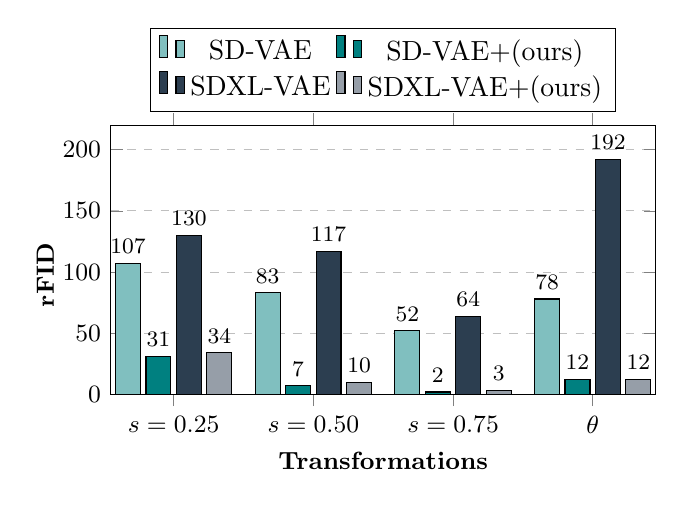
\begin{tikzpicture}
        \begin{axis}[
            ybar,
            width=8.5cm,
            height=5cm,
            bar width=9pt,
            ymin=0,
            ymax=220,
            ylabel={\Th{\textbf{rFID}}},
            y label style={
                at={(axis description cs:-0.12,0.6)}, % Adjust the position
                anchor=east                         % Align the label properly
            },
            xlabel={\textbf{Transformations}},
            symbolic x coords={$s=0.25$,$s=0.50$,$s=0.75$,$\theta$},
            xtick=data,
            ymajorgrids=true,
            grid style=dashed,
            enlarge x limits=0.15,
            legend style={
                at={(0.5,1.05)},
                anchor=south,
                legend columns=2,
            },
            nodes near coords,
            every node near coord/.append style={font=\footnotesize, anchor=south},
            label style={font=\small},
            ticklabel style={font=\small},
        ]
        
        % SD-VAE
        \addplot [
            fill=SDVAE!50, 
            draw=black, 
        ] coordinates {
            ($s=0.75$, 52)
            ($s=0.50$, 83)
            ($s=0.25$, 107)
            ($\theta$, 78)
        };
        
        % SD-VAE+(ours)
        \addplot [
            fill=SDVAE, 
            draw=black, 
        ] coordinates {
            ($s=0.75$, 2)
            ($s=0.50$, 7)
            ($s=0.25$, 31)
            ($\theta$, 12)
        };
        
        % SDXL-VAE
        \addplot [
            fill=SDXLVAE, 
            draw=black, 
        ] coordinates {
            ($s=0.75$, 64)
            ($s=0.50$, 117)
            ($s=0.25$, 130)
            ($\theta$, 192)
        };
        
        % SDXL-VAE+(ours)
        \addplot [
            fill=SDXLVAE!50, 
            draw=black, 
        ] coordinates {
            ($s=0.75$, 3)
            ($s=0.50$, 10)
            ($s=0.25$, 34)
            ($\theta$, 12)
        };
        
        \legend{SD-VAE, SD-VAE+(ours), SDXL-VAE, SDXL-VAE+(ours)}
        
        \end{axis}
    \end{tikzpicture}
    \caption{\textbf{Enhanced Reconstruction under Latent Transformations.} Reconstruction \Th{rFID} measured between $\tau \circ \mathbf{x}$ and $ \mathcal{D}(\tau \circ \mathcal{E}(\mathbf{x}))$ for various spatial transformations. We consider scaling transforms with factors $s = 0.75, 0.50, 0.25$ and also measure the average \Th{rFID}  over rotation angles $\theta = \frac{\pi}{2}, \pi, \frac{3\pi}{2}$. Results for \sdvae~\cite{rombach2022high} and \texttt{SDXL-VAE}~\cite{podell2024sdxl}, with and without \our. Our approach significantly reduces \Th{rFID} compared to baselines, improving image fidelity under latent transformations. For readability, we show $\floor{\Th{rFID}}$. }
    \label{fig:scales-rfig}
\end{figure}